\chapter{Background}\label{cha:background}

The following chapter lays the theoretical groundwork for the project. An understanding of linear algebra, numerical optimization, algorithms, and statistics is assumed. 

\section{Mathematical Programming}

In this project, the terms mathematical programming, numerical optimization, and optimization are used interchangeably.


\subsection{Linear Programming}

In mathematical programming, the general linear problem can be stated as \cite{gasse2019exact}:
\begin{align} \label{eq:lp}
    \underset{\mathbf{x}}{\arg \min }\left\{\mathbf{c}^{\top} \mathbf{x} \; \mid \mathbf{A} \mathbf{x} \leq \mathbf{b},\; \mathbf{x} \in \mathbb{R}_+^{n}\right\},
\end{align}
where $ \mathbf{x} \in \mathbb{R}_+^n$ is the variable vector
with the objective coefficient vector $c \in R^n $, 
the constraint coefficient matrix $\mathbf{A} \in R^{m \times n}$
and the constraint right-hand-side vector $b \in R^m $.

The size of the problem will be measured by the dimensions of the constraint coefficient matrix $ \mathbb{A} $, where the number of rows and columns corresponds to the number of variables and constraints, respectively.

These problems are convex \cite{wolsey2020integer}, and can be solved by several efficient algorithms. The simplex algorithm can solve problems on this form efficiently, as optimal points are guaranteed to be on the vertices of the feasible set, and the same for interior-point methods \cite{nocedal2006numerical}. These algorithms are good average performance but do not have guaranteed polynomial running time in the worst case. Guaranteed polynomial solution algorithms do exist, for instance Karamkar's algorithm \cite{karamkar1984new}. 


\subsection{Mixed Integer Linear Programming}

Mixed Integer Linear Programming is a superset of linear programming, where one or more of the variables can be restricted to discrete values. The general problem can in this case be stated as \cite{gasse2019exact}:
\begin{align}\label{eq:milp}
    \underset{\mathbf{x}}{\arg \min }\left\{\mathbf{c}^{\top} \mathbf{x} \mid \mathbf{A} \mathbf{x} \leq \mathbf{b}, \; \mathbf{x} \in \mathbb{Z}_+^{p} \times \mathbb{R}_+^{n-p}\right\},
\end{align}
where $ p $ is the number of integer variables, otherwise the variables are the same as \Cref{eq:lp}.

% https://texample.net/tikz/examples/colored-diagram/
\begin{figure}
    \centering
    \begin{tikzpicture}[
        thick,scale=0.5, 
        every node/.style={scale=0.2}
        every path/.style = {},
        every node/.append style = {font=\sffamily}
      ]
      \begin{scope}
        \shade[right color=gray, left color=white, opacity=0.7]
          (-0.5,-0.5) rectangle (0,6.5);
        \node[rotate=90, above] at (0,3) {};
        \shade[top color=gray, bottom color=white, opacity=0.7]
          (-0.5,-0.5) rectangle (8.5,0);
        \shade[left color=gray, bottom color=gray, right color=white, opacity=0.5]
          (-0.5,5.5) -- (8.5,3) -- (8.5,6.5) -- (-0.5,6.5) -- cycle;
        \path (-0.5,5.5) -- node[pos=0.23, sloped, above] {}
          (8.5,3);
        \shade[left color=gray, right color=white, opacity=0.5]
          (2.5,6.5) -- (8.5,6.5) -- (8.5,0) -- (5,0) -- cycle;
        \path (5,0) -- node[pos=0.3, sloped, above] {} (2.5,6.5);
        \node[text width=6em, align=center] at (2,2)
          {};
        \draw[->] (-0.5,0) -- (8.5,0) node[below] {x};
        \draw[->] (0,-0.5) -- (0,6.5) node[above] {y};
        \node[rotate=-45, above, text width=9em, align=center] at (7.25,5.25)
          {};
        \path[clip] (-0.5,-0.5) rectangle (8.5,6.5);
        \foreach \i in {0.5,3,...,13} {
          \draw[help lines] (-0.5,\i) -- +(-45:15);
        }
      \end{scope}
      \draw[very thick, ->] (9,3.25) -- node[above, text width=3cm, align=center]
        {} (11.5,3.25);
      \begin{scope}[shift={(13,0)}]
        \shade[right color=gray, left color=white, opacity=0.7]
          (-0.5,-0.5) rectangle (0,6.5);
        \shade[top color=gray, bottom color=white, opacity=0.7]
          (-0.5,-0.5) rectangle (8.5,0);
        \shade[left color=gray, bottom color=gray, right color=white, opacity=0.5]
          (-0.5,5.5) -- (8.5,3) -- (8.5,6.5) -- (-0.5,6.5) -- cycle;
       \shade[left color=gray, right color=gray, opacity=0.5]
         (2.5,6.5) -- (8.5,6.5) -- (8.5,0) -- (5,0) -- cycle;
        \draw[->] (-0.5,0) -- (8.5,0) node[below] {x};
        \draw[->] (0,-0.5) -- (0,6.5) node[above] {y};
        \foreach \i in {0,1,...,6.5} {
          \draw[help lines] (-0.5,\i) -- (8.5,\i);
        }
        \foreach \i in {2,4,...,8.5} {
          \draw[help lines] (\i,6.5) -- (\i,-0.5);
        }
        \foreach \i in {0,1,...,5} {
          \node[draw,cross out,label={left:\i}] at (0,\i) {};
        }
        \foreach \i in {0,1,...,4} {
          \node[draw,cross out] at (2,\i) {};
        }
        \foreach \i in {0,1,...,2} {
                \node[draw,cross out] at (4,\i) {};
        }
        \foreach \i in {0,2,...,6} {
          \node[below] at (\i,0) {\pgfmathparse{int(\i/2)}\pgfmathresult};
        }
      \end{scope}
    \end{tikzpicture}
    \caption{Figure of an \Gls{LP} and the corresponding \Gls{ILP}}
    \label{fig:milpfig}
\end{figure}

In \Cref{fig:milpfig}, an \gls{LP} problem and the problem with integrality constraints is shown. For the LP problem, the shaded areas represent the inequality constraints, where the diagonal lines represent the level curves of the objective function. In the \gls{ILP} problem, the crosses represent the feasible solutions. The LP is also called a \textit{relaxation} of the original \gls{ILP}, which is fundamental to efficient solving algorithms of \gls{MILP} problems.

A problem that includes integrality constraints cannot be convex \cite{wolsey2020integer}. The non-convexity of the feasible set of the problem constitutes a significant challenge, and it is considered unlikely that polynomial-time solutions exist \cite{papadimitriou1982combinatorial}. \gls{MILP} problems belong to the category of \gls{NP}-hard problems \cite{papadimitriou1982combinatorial}.   



A subset of \gls{MILP} problems can be Integer Linear Programming (\gls{ILP}), where all variables are restricted to integer values, or Binary Linear Programming (\gls{BLP}), where all variables are restricted to binary values. 

\gls{ILP} and \gls{BLP} problems belong to the category of combinatorial optimization problems, which has been the main focus of the efforts to solve entirely or partially with machine learning methods \cite{bengio2020machine}. 


\section{Branch and Bound}\label{sec:bnb}

A \textit{relaxation} of a \gls{MILP} problem is achieved by relaxing the integrality constraint, as shown in \Cref{fig:milpfig}. Obtaining the solution to the relaxed problem gives a lower bound on the optimal solution (for a minimization problem). Naturally, any feasible solution to the integrality-constrained problem gives an upper bound on the solution. Furthermore, if the solution to the relaxed problem adheres to the integrality constraints, it is also the solution to the MILP problem \cite{wolsey2020integer}.

The most prevalent solution algorithm for MILP problems exploits these results, by sequentially dividing the solution space until the optimum with the integrality constraint is found. This is done by branching in a bipartite graph according to \cite{gasse2019exact}:
\begin{align} \label{eq:branch}
    x_{i} \leq\left\lfloor x_{i}^{\star}\right\rfloor \vee x_{i} \geq\left\lceil x_{i}^{\star}\right\rceil, \quad \exists \; i \leq p \mid x_{i}^{\star} \notin \mathbb{Z}    
\end{align}
Further creating sub-problems with this binary decomposition. An illustration of this process is shown in \Cref{fig:bandb1}.

%https://tex.stackexchange.com/questions/416359/branch-and-bound-tree-in-tikz
\comments{
\begin{figure}
\centering
\begin{forest}
  branch and bound,
  where level=1{
    set branch labels={x\leq}{}{x\geq}{},
  }{
    if level=2{
      set branch labels={}{\geq y}{}{\leq y},
    }{},
  }
  [1055.56:S:950
    [1000:S_1:950:5
    ]
    [1033:S_2:950:6
      [1033:{S_2,1}:950:1]
      [950:{S_2,2}:1033:2]
    ]
  ]
\end{forest}
\caption{\label{fig:bandb1}PLACEHOLDER Illustration of the branch and bound algorithm}
\end{figure}}

\begin{figure}
\centering
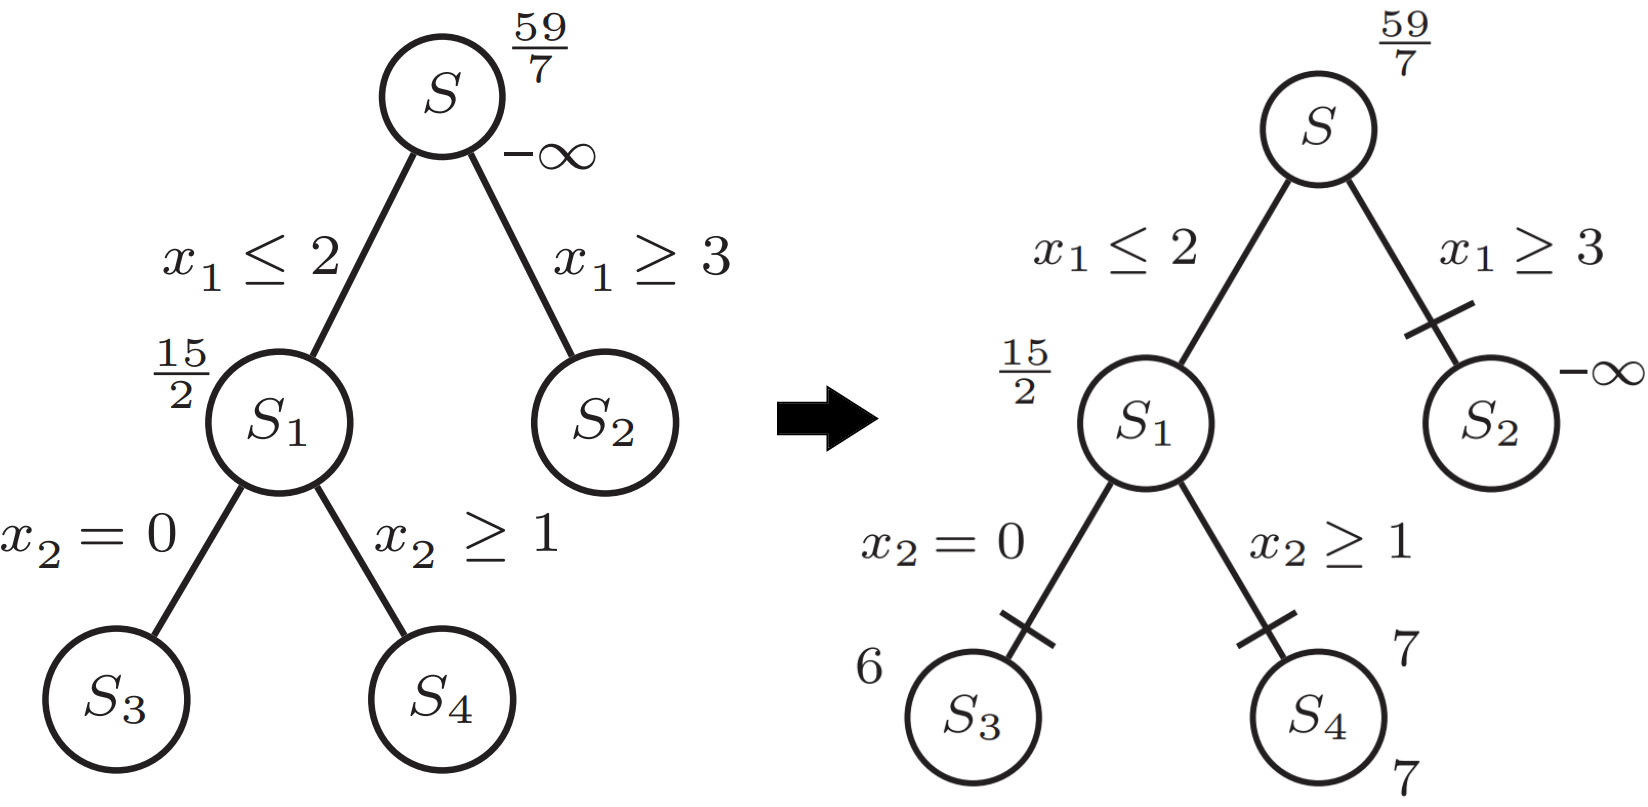
\includegraphics[width=0.8\linewidth]{img/bnb.png}
\caption{\label{fig:bandb1}Illustration of the branch and bound algorithm adapted from a maximization problem in \textit{Integer Programming }(2020) \cite{wolsey2020integer}}
\end{figure}

For each generated solution, represented by nodes in \Cref{fig:bandb1}, a relaxation of the problem is solved in order to obtain an upper and lower bound on the solution of the sub-problem. 
These values are shown on the top and bottom right, respectively. 
Generating upper and lower bounds for solutions allow for discarding a large number of solutions \cite{wolsey2020integer}. Branches can be \textit{pruned} (meaning no further partitioning from that branch) if they meet at least one of the following three criteria \cite{wolsey2020integer}:
\newpage
\begin{enumerate}[label=(\roman*)]
    \item Pruning by optimality: $Z^t = \{\max \bm{c}^{\top} \bm{x} : \bm{x} \in S_t\}$ has been solved.
    \item Pruning by bound: $\overline{Z}^t \leq \underline{Z}^t$.
    \item Pruning by infeasiblity: $S_t = \emptyset $.
\end{enumerate}
For \Cref{fig:bandb1}, the graph on the right represents the tree after solving the relaxation, resulting in $S_2$ being pruned by infeasibility, $S_3$ cut off by bound and $S_4$ pruned by optimality.


The choice of node and variable to branch on to find the optimum in the fewest number of branching processes is central to an efficient implementation of \gls{BnB}. Partitioning the feasible set such that the node with the optimal value (criteria i) is found in the fewest possible branchings is the optimal strategy. 


\subsection{Valid Inequalities}\label{ssec:inequalities}

Another important method used in \gls{BnB} algorithms is the concept of valid inequalities. A valid inequality is an inequality that does not remove feasible solutions of the non-convex solution set but can remove potential solutions to the relaxed problems. A valid inequality can be expressed as:
\begin{equation}\label{eq:cut}
    \bm{\pi}^{\top} \bm{x} \leq \pi_0 \quad \forall \; \mathbf{x} \in  \bm{X}   
\end{equation}
where $\bm{X}$ is the feasible set as described in \Cref{eq:milp}. These inequalities reduce the size of the feasible set for the relaxations of the problem without removing feasible solutions of the original problem. An illustration of an \gls{ILP} with an added valid inequality is shown in \Cref{fig:cut}. Here the feasible set of the relaxation is reduced in size by the added constraint, while the feasible points of the \gls{ILP} remain feasible after the application of the inequality, as is given in \Cref{eq:cut}.

\begin{figure}
    \centering
    \begin{tikzpicture}[
        thick,scale=0.5, 
        every node/.style={scale=0.2}
        every path/.style = {},
        every node/.append style = {font=\sffamily}
      ]
      \begin{scope}
        \shade[right color=gray, left color=white, opacity=0.7]
          (-0.5,-0.5) rectangle (0,6.5);
        \shade[top color=gray, bottom color=white, opacity=0.7]
          (-0.5,-0.5) rectangle (8.5,0);
        \shade[left color=gray, bottom color=gray, right color=white, opacity=0.5]
          (-0.5,5.5) -- (8.5,3) -- (8.5,6.5) -- (-0.5,6.5) -- cycle;
       \shade[left color=gray, right color=gray, opacity=0.5]
         (2.5,6.5) -- (8.5,6.5) -- (8.5,0) -- (5,0) -- cycle;
        \draw[->] (-0.5,0) -- (8.5,0) node[below] {x};
        \draw[->] (0,-0.5) -- (0,6.5) node[above] {y};
        \foreach \i in {0,1,...,6.5} {
          \draw[help lines] (-0.5,\i) -- (8.5,\i);
        }
        \foreach \i in {2,4,...,8.5} {
          \draw[help lines] (\i,6.5) -- (\i,-0.5);
        }
        \foreach \i in {0,1,...,5} {
          \node[draw,cross out] at (0,\i) {};
        }
        \foreach \i in {0,1,...,4} {
          \node[draw,cross out] at (2,\i) {};
        }
        \foreach \i in {0,1,...,2} {
                \node[draw,cross out] at (4,\i) {};
        }
      \end{scope}
      \draw[very thick, ->] (9,3.25) -- node[above, text width=3cm, align=center]
        {} (11.5,3.25);
      \begin{scope}[shift={(13,0)}]
        \shade[right color=gray, left color=white, opacity=0.7]
          (-0.5,-0.5) rectangle (0,6.5);
        \shade[top color=gray, bottom color=white, opacity=0.7]
          (-0.5,-0.5) rectangle (8.5,0);
        \shade[left color=gray, bottom color=gray, right color=white, opacity=0.5]
          (-0.5,5.5) -- (8.5,3) -- (8.5,6.5) -- (-0.5,6.5) -- cycle;
        \shade[left color=gray, right color=gray, opacity=0.5]
          (2.5,6.5) -- (8.5,6.5) -- (8.5,0) -- (5,0) -- cycle;
        \shade[left color=gray, right color=gray, opacity=0.5]
          (0.0,6.5) -- (8.5,6.5) -- (8.5,0) -- (6.0,0) -- cycle;
        \draw[->] (-0.5,0) -- (8.5,0) node[below] {x};
        \draw[->] (0,-0.5) -- (0,6.5) node[above] {y};
        \foreach \i in {0,1,...,6.5} {
          \draw[help lines] (-0.5,\i) -- (8.5,\i);
        }
        \foreach \i in {2,4,...,8.5} {
          \draw[help lines] (\i,6.5) -- (\i,-0.5);
        }
        \foreach \i in {0,1,...,5} {
          \node[draw,cross out] at (0,\i) {};
        }
        \foreach \i in {0,1,...,4} {
          \node[draw,cross out] at (2,\i) {};
        }
        \foreach \i in {0,1,...,2} {
                \node[draw,cross out] at (4,\i) {};
        }
      \end{scope}
    \end{tikzpicture}
    \caption{Figure of \Gls{ILP} before and after an added valid inequality.}
    \label{fig:cut}
\end{figure}
 


Algorithms that find these inequalities during the \gls{BnB} algorithm are called \textit{Branch and Cut}. The nomenclature comes from calling the application of these inequalities \textit{cuts} or \textit{cutting planes}.
When an application of inequalities are only employed on the root node (before dividing the solution space in the enumeration), the algorithm is sometimes referred to as \textit{Cut and Branch} rather than \textit{Branch and Cut} \cite{wolsey2020integer}.

\subsection{Primal and Dual Heuristics}

The efficiency of modern \gls{MILP} solvers rely on their implementation of \textit{primal} and \textit{dual} heuristics.

Primal heuristics are methods for finding feasible solutions at a given \gls{BnB} node, where the quality, or distance to the optimal bound, is the determining factor to whether the feasible solution is useful or not \cite{khalil2020towards}. These heuristics are as costly as they are useful, and modern solvers periodically run different heuristics at different times during the solution process \cite{khalil2020towards}.  

Dual heuristics are the backbone of the creation of the \gls{BnB} tree. This includes selecting which node to branch from, and which variable to branch on at the selected node CHECK!!. The application of cutting planes is also classified under dual heuristics.


\subsection{Branching Variable Selection Strategy}\label{ssec:branchingstrategy}

As mentioned, an important decision in the B\&B algorithm is the choice of the variable that should be branched on. 
There exists many heuristics for solving this, which vary in computational complexity and accuracy. 
A good branching algorithm should choose to branch on variables that lead to small solution trees (fewer nodes evaluated) and find these variables in a computationally efficient manner. 

The current branching strategy resulting in the smallest solution trees is known as \textit{Strong Branching} (\gls{SB}) \cite{applegate1995finding}, and the application of this branching strategy at every node is known as \textit{Full Strong Branching} (\gls{FSB}) \cite{achterberg2004branching}. 
This branching policy is based on determining the best variable to branch on by solving the relaxation for every candidate variable and is therefore very computationally expensive compared to other methods \cite{achterberg2004branching}.

All popular variable selection strategies depend on scoring all the possible variables and selecting the variable with the most optimal score \cite{achterberg2004branching}. There are two other classes of branching strategies than \gls{FSB}: \textit{Most Infeasible Branching} (\gls{MIB}), where the variable with the fractional part of the relaxation optimum closest to $0.5$ is selected (a very poor strategy) 
and \textit{Pseudo-cost Branching} (\gls{PB}), which relies on the expected change in objective value based on previous branching on the variable in question
\cite{achterberg2004branching}. Today, combinations of \gls{FSB} and \gls{PB} are most common \cite{anand2017comparative}.   

In the literature, the branching strategy is referred to as a strategy, policy, or rule, in this project \textit{strategy} is used.  


\section{Learned Branching Policy}

Recently, attempts have been made to find a branching strategy based on statistical learning. 

Using machine learning, specifically imitation learning, to find good candidate variables for branching in a less computationally demanding manner was proposed by Elias Khalil \cite{khalil2016learning}. Various methods for learning in branching include \textit{ Support Vector Machine Ranking} (\Gls{SVM}) \cite{khalil2016learning}, \textit{Graph Convolutional Neural Networks} (\gls{GCNN}) \cite{gasse2019exact} and \textit{Feature-wise Linear Modulation} (\gls{FiLM}) \cite{gupta2020hybrid}.

The fundamental assumption to this approach is that the most computationally demanding but most accurate branching policy can be learned. The algorithm will use imitation learning on the branching expert to find a computationally less expensive non-linear function approximation to the expert algorithm's variable scoring. Then, the algorithm branches on the variable with the highest score. This can be expressed as: 
\begin{align}
    f(i) &=  \pi_{SB} (i) + \epsilon \quad \forall \; i \in \mathcal{C}\\
    f(i) &= s_i\\
    i^*_f &= \underset{i \in \mathcal{C}}{\mathrm{argmin}} \; \bm{s}_i
\end{align}
where $f$ is the learned function, $\mathcal{C}$ is the set of possible branching variables, $\pi_{SB}$ is the Strong Branching strategy and $\epsilon$ is the deviation in the scoring function. 


\section{Multi-layer Perceptrons}

Multi-Layer Perceptrons (MLP), more commonly known as deep feed-forward neural networks, are recommended by Gupta et al. (2020) \cite{gupta2020hybrid} as a less computationally expensive alternative to the approaches by Khalil et al. (2016) \cite{khalil2016learning} and Gasse et al. (2019) \cite{gasse2019exact}. 

MLPs are networks that generate a nonlinear function $y = f(\mathbf{x}; \bm{\theta})$, where $x$ is the input $y$ is the output and $\bm{\theta}$ represents the parameters of the function. The parameters are learned during repeated optimization, and will under ideal circumstances converge to approach the goal function $y = f^*(\mathbf{x})$. The function is realized as a series of compositions of functions. The composed functions are represented as an acyclical, directed graph \cite{nielsen2018neural}, and can be expressed as:
\begin{align}
    y = f_L \circ f_{L-1} \circ \ldots \circ f_{1} \circ f_{0} (\mathbf{x})  
\end{align}
The functions are denoted as layers of the perceptron, and are implemented as affine functions of every input parameter at every node, $\mathbf{z}_l = \mathbf{x}_{l-1}^T \mathbf{w}_l + \mathbf{b}_l$. Applying non-linear function, known as an \textit{activation function}, allows the \gls{MLP} to represent arbitrary nonlinear functions \cite{goodfellow2016deep}. This is expressed as $\mathbf{x}_l = \mathbf{a}(\mathbf{z}_l)$.

The computation of the output of the function given its input is known as a \textit{forward pass} through the network. The required computations for a single input vector into a network with $ n $ hidden layers will include $ n + 1 $ matrix multiplications and $ n + 1 $ applications of the non-linear activation function, given that there is an activation function on the output. 

Depending on the training configuration, the problem can be interpreted as a classification problem or regression problem (or a ranking problem, as in \cite{khalil2016learning}). In the following experiments, the former approach is selected, as has become popular after Gasse et al. (2019) \cite{gasse2019exact}. 





\section{Markov Decision Processes}\label{sec:mdp}

Central to the advancement of learned strategies in \gls{BnB} is the interpretation of the solution algorithm as a \textit{Markov Decision Process} (\gls{MDP}) \cite{gasse2019exact}. This interpretation relates the problem to a large collection of literature on the topic \cite{howard1960dynamic}.

An \gls{MDP} is expressed as $ \mathcal{S}, \mathcal{A}, p_{init}, p_{trans}, R$ 
where $ \mathcal{S}$ is the state space, 
$\mathcal{A}$ is the action space, 
$p_{init}$ is an initial state distribution ($p_{init}\;:\;\mathcal{S}\leftarrow \mathbb{R}_{\geq 0}$), 
$p_{trans}$ is the state transition distribution (
$p_{trans}\; : \; \mathcal{S}
\times \mathcal{A}\times \mathcal{S}
\leftarrow \mathbb{R}_{\geq 0}$), 
$p_{trans}$), $R$ is the reward function $R\;:\;\mathcal{S} \rightarrow \mathbb{R}$. \cite{prouvost2020ecole}. 

Further, the \textit{action policy} $\pi$ is given as $\pi \; : \; \mathcal{A}\times \mathcal{S}
\leftarrow \mathbb{R}_{\geq 0}$, and results in state-action trajectories $\tau = (s_0, a_0, s_1, a_1, ... )$ that obey a joint distribution that can be expressed as following: \cite{prouvost2020ecole}
\begin{equation}
    \tau \sim \underbrace{p_\textit{init}(s_0)}_{\text{initial state}}
\prod_{t=0}^\infty \underbrace{\pi(a_t | s_t)}_{\text{next action}}
\underbrace{p_\textit{trans}(s_{t+1} | a_t, s_t)}_{\text{next state}}
\end{equation}

These definitions now allow a formulation of the \gls{MDP} control problem, which is the problem of interest in this thesis. The control problem consists of finding the action policy that maximizes the reward, and can be stated as: \cite{prouvost2020ecole}
\begin{equation}\label{eq:mdprcontrol}
    [\pi^\star = \underset{\pi}{\operatorname{arg\,max}}
\lim_{T \to \infty} \mathbb{E}_\tau\left[\sum_{t=0}^{T} R(s_t)\right]
\end{equation}


\subsection{Partially-observable Markov Decision Processes}

A subset or generalization of an \gls{MDP} is the \textit{Partially-observable Markov Decision Process }(\gls{PO-MDP}) \cite{monahan1982state}. Processes of this class allows for uncertainty of the states as well as additional acquisition of state information \cite{monahan1982state}.
The addition of an observation of the process in the observation space ($o \in \Omega $) extends the process to the formulation to $ (\mathcal{S}, \mathcal{A}, p_{init}, p_{trans}, R, O)$. 

The generalization from \gls{MDP} to \gls{PO-MDP} concedes the Markovian nature of the trajectories \cite{prouvost2020ecole}, i.e:
\begin{equation}
    o_{t+1},r_{t+1} \not \perp   h_{t-1} \mid o_t,r_t,a_t
\text{,}
\end{equation}
meaning that the entire action-state history of the process is necessary for the policy. The history is denoted $\mathcal{H}$, and the policy of the \gls{PO-MDP} is stated as:
\begin{equation}
    \pi:\mathcal{A} \times \mathcal{H} \to \mathbb{R}_{\geq 0}
\end{equation}
which means that the control problem of the \gls{PO-MDP} can also be stated as \cref{eq:mdprcontrol}.

\subsection{Branch \& Bound as a \gls{PO-MDP}}

Interpreted in the language of \gls{MDP}s, the \gls{BnB} algorithm is the \textit{environment} and a concrete \gls{MILP} problem instance is an \textit{episode} in this environment. The \textit{agent} is the brancher, where in this thesis the variable selection policy is the component of interest, ignoring the node selection policy. The state of the solver consists of the \gls{BnB} tree at that instance, as well as the observations at each node (the \textit{history} of the \gls{PO-MDP}).

This formulation is the basis for the \textit{Ecole} framework, which is discussed in \Cref{sec:ecole}
The \gls{PO-MDP} formulation allows for the agent in the \gls{BnB} environment to be learned through \textit{reinforcement learning}


\section{Reinforcement Learning}

The subset of machine learning described as Reinforcement Learning (\gls{RL}) is highly relevant in the context of \gls{ML} in \gls{CO}. No results will be discussed in this thesis, however a background in the topic is necessary to understand both other works in the field and the long-term goals of the project.

\gls{RL} encompasses the problem of an \textit{agent} learning a \textit{policy} for behaving in an \textit{environment} so as to achieve a global objective. Any sequential decision-making problem with a measure of optimality that relies on past experience can be formulated as a \gls{RL} problem \cite{francois2018introduction}. In addition, the approach has seen success in a number of fields in the past years with the integration of deep learning models, often termed deep \gls{RL} \cite{francois2018introduction}. Most notable of the advancements might be AlphaZero, Google's successful chess-AI \cite{silver2017mastering}. \gls{RL} has the important property of being independent of data, meaning a number of core \gls{ML} challenges (quantity, quality, and bias of data) are rendered irrelevant. 

\gls{RL} is particularly interesting in \gls{BnB} because of the \gls{MDP} nature of the algorithm, and the assumption that the handcrafted heuristics and sub-algorithms prevalent in modern solvers are either inefficient or inaccurate compared to the theoretical capabilities of, i.e. neural networks. 

Many attempts have been made at implementing \gls{RL} in \gls{CO}, see for example Etheve et al. (2020) \cite{etheve2020reinforcement} or Tang et al. (2020) \cite{tang2020reinforcement}. Approaches for learning variable selection, such as reported in Scavuzzo (2020) \cite{scavuzzo2020learning}, rely on efficient and accurate pre-trained models based on imitation learning, like the models presented in this thesis. More knowledge is likely needed for the pure \gls{RL} approach to take over the mantle.
\footnote{Attempts on \gls{RL} models were also made by the author of this thesis, but the models did not prove useful with the chosen method and are therefore not reported.}
Cappart et al. (2021) \cite{cappart2021combinatorial} also conclude that useful \gls{RL} policies are not mature yet. 






\section{Graph Convolutional Neural Networks }

Graph Convolutional Neural Networks (\gls{GCNN}s) is a term for neural networks that have input data represented in a graph-structure that is processed by the convolution operation \cite{kipf2016semisupervised}. The graph convolution operation is defied by the propagation rule \cite{kipf2016semisupervised}:
\begin{equation}
    H^{(l+1)} = \sigma \left( \Tilde{D}^{-\frac{1}{2}} \Tilde{A} \Tilde{D}^{-\frac{1}{2}} H^{(l)}W^{(l)}\right)
\end{equation}
where $H^{(l)}$ is the matrix of activations in layer $l$ (meaning $H^{(0)} = 0$). $\Tilde{A} = A + I_N$, where $A$ is the adjacency matrix representing the undirected graph $\mathcal{G}$, and $\Tilde{D} = \sum_j \Tilde{A}_{i j}$. $\sigma( \cdot) $ is a nonlinear activation function.
This operation is shown to be inspired by the first order approximations to spectral filters on graphs \cite{kipf2016semisupervised}.

The term \textit{embeddings} will be used in this thesis for continuous-variable representations derived from the input features, as it is used in Gasse et al. \cite{gasse2019exact}. 

Models that leverage the graph nature of combinatorial optimization problems have been shown to have satisfactory performance, see e.g. Dai et al. (2018) \cite{dai2018learning}. 
\gls{GCNN}s are proposed by Gasse et al. \cite{gasse2019exact} as an alternative to the feature-rich approaches by Khalil et al. (2016) \cite{khalil2016learning}. 
The application of \gls{GCNN}s on \gls{BnB} algorithms relies on the bipartite graph structure that results from the solution process, as explained in \Cref{sec:bnb}. At each point before the variable selection process, the state of the solution algorithm graph can be processed by the \gls{GCNN} algorithm. 

The state of the \gls{BnB} graph at a node can be represented as $s_t = (\mathcal{G}, \mathbf{C}, \mathbf{E}, \mathbf{V})$, where $\mathcal{G}$ represents the bipartite \gls{BnB} solution graph at that time instance, $\mathbf{C}$ represents the constraints, $\mathbf{E}$ represents the \textit{edges}, or connections between the variables and constraints, and $\mathbf{V}$ represents candidate variables.  